\section{Experimental Evaluation}
\subsection{Protocol and Scope}
We report four completed studies: RTL acquisition, frozen repair transfer, physical-data conversion, and downstream prediction. Each study uses a dedicated cohort and reports its own acceptance endpoint. The acquisition toolchain is pinned to ORFS commit \texttt{a5ff7ef7}, Yosys 0.64, and OpenROAD \texttt{26Q3-318-g6b9d7fb806}; individual campaigns retain their own runtime and protocol manifests. Models are identified by their full version names throughout.

\subsection{Qualified RTL Acquisition}
Each method receives four CPU cores, one concurrent synthesis job, and a 48-hour wall-clock ceiling. Tool-enabled vanilla LLMs additionally have ceilings of 20 million tokens, 1,600 turns, and 960 search requests. The LLM roster is GPT-5.6-sol, Claude Opus 5, Qwen3.7-Max, Kimi-K2.7-Code, DeepSeek-V4-Pro, grok-4.5, and Gemini-3.1-Pro-Preview. R2G starts with empty search-scheduling state and uses no external LLM tokens. All methods are evaluated after their submissions are locked, using fresh source retrieval and independent synthesis. Confirmed infrastructure failures can be retried on unchanged submissions; actual qualification failures cannot be replaced after scoring.

\begin{figure}[htbp]
\centering
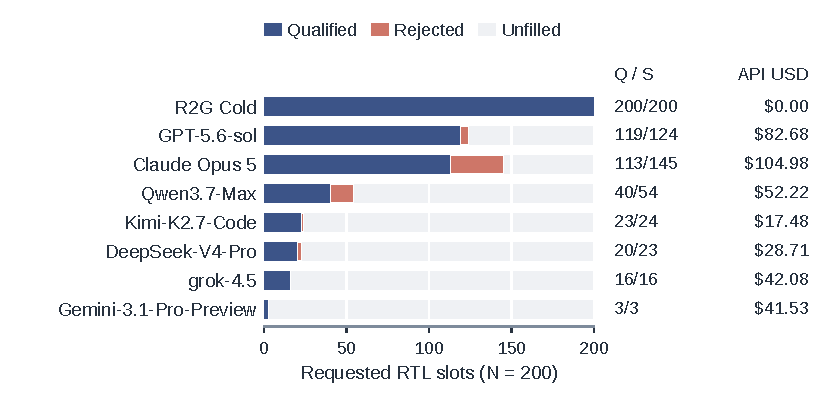
\includegraphics[width=\linewidth]{figures/acquisition_yield.pdf}
\caption{Qualified RTL acquisition under the campaign budgets. Each bar represents 200 requested slots; Q/S gives qualified/submitted counts. Coral denotes rejected submissions; gray denotes unfilled slots. R2G takes 33.52 h. API USD gives reference-price estimates (Appendix~\ref{app:api_costs}).}
\label{fig:acquisition}
\end{figure}

R2G supplies all 200 qualified designs, exceeding GPT-5.6-sol by 81 designs, or 40.5 percentage points of fixed-target yield (Fig.~\ref{fig:acquisition}). Its qualified set spans 122 repositories, compared with 70 for GPT-5.6-sol and 52 for Claude Opus 5, with a maximum single-repository contribution of 2\%. The acquisition bottleneck is not solely submitted-candidate accuracy: GPT-5.6-sol qualifies 119 of 124 submissions, yet leaves 76 slots unfilled. Results are measured per budgeted acquisition campaign.

R2G completes the target in 33.52 hours. The recorded LLM runs take 2.28--10.58 hours and stop at token or turn ceilings, so the comparison measures final qualified yield under the stated budgets. Infrastructure-only reevaluation raises R2G's count from 195 to 200 using the same five submissions; equivalent retry rules apply to the other methods.

\subsection{Repair Transfer and Full-System Evaluation}
The repair cohort contains six proposal challenges, six validation challenges, and 13 held-out challenges: seven DRC and six setup-timing cases. Four baseline-clean sentinels are separate from the repair denominator. Splits prohibit shared repositories, forks, compilation closures, or RTL lineages across subsets. M0--M3 use the prescribed development split; Full R2G uses the complete Recipe library, including recipes developed using evidence from the evaluated challenge set. Every ORFS trial uses four cores and a 7,200-second ceiling at fixed Sky130HD, 100 MHz. GPT-5.6-sol, Claude Opus 5, and Qwen3.7-Max repair each held-out challenge independently with the same permitted actions, up to three response turns and 20,000 tokens per model per challenge.

\begin{figure}[htbp]
\centering
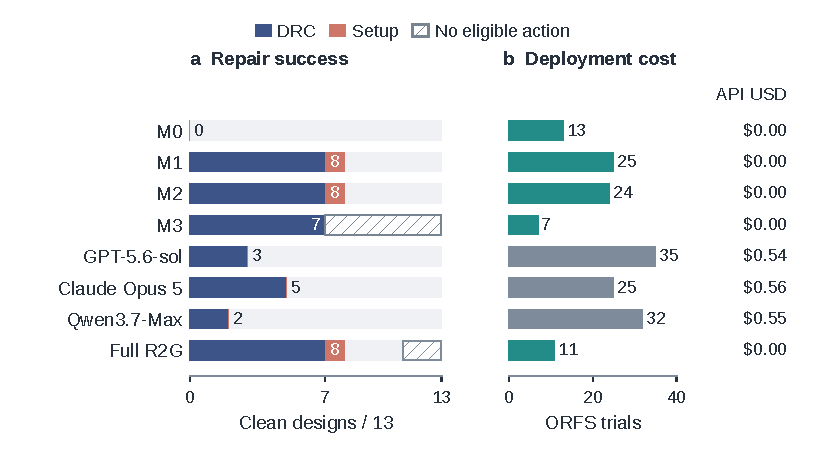
\includegraphics[width=\linewidth]{figures/repair_outcomes_cost.pdf}
\caption{Repair outcomes and deployment cost. Blue/coral count DRC/setup successes out of 13 challenges; gray denotes unsuccessful attempts and hatching no eligible action. Trial counts and estimated API USD cover deployment; the shared proposal phase costs \$0.57 (Appendix~\ref{app:api_costs}).}
\label{fig:repair}
\end{figure}

Seventeen structured records produce ten admitted candidates and three promoted records, corresponding to two distinct executable recipes. Both target the \texttt{DRC:m3.2} edge-pin congestion family: one excludes right-edge pin placement; the other combines hierarchical synthesis with top-edge exclusion. No setup-timing candidate is promoted.

M1 and M2 each repair eight held-out challenges, three more than the strongest pure LLM baseline, Claude Opus 5 (Fig.~\ref{fig:repair}). They reach the same successful design set, with M2 using 24 trials and M1 using 25. M3 repairs seven of 13 challenges overall and seven of seven covered challenges, using one trial per covered case. The promoted policy uses seven trials and abstains on the six setup challenges. M1, M2, and M3 retain strict-clean outcomes on all four tested sentinels.

M1/M2 require 40,460.063/40,919.486 accumulated EDA seconds on the held-out challenges; M3 requires 6,500.894 seconds. These costs sum the individual trial durations. Held-out R2G execution consumes no LLM tokens, but the proposal phase costs 109,236 tokens and 18 calls. The formal A replays also consume 110 ORFS attempts (77 proposal and 33 validation attempts), excluding other learning work. Learning and deployment costs are accounted for separately. The pure-LLM held-out runs consume 207,442 tokens in aggregate.



These results characterize transfer on the seven DRC and six setup challenges. An exploratory paired comparison of M1 and Claude Opus 5 gives three wins unique to M1 and none unique to Claude Opus 5 (two-sided exact McNemar $p=0.25$).

\textbf{Full R2G.} We evaluate a frozen snapshot of the complete native Recipe library on the same 13 challenges, preserving RTL, clock, floorplan, and strict checks. Native ranking and lifecycle gates select actions through the budgeted configuration adapter. Full R2G achieves \textbf{8/13 strict-clean designs (61.54\%)}: seven DRC and one setup case, using \textbf{11 repair trials} with no evaluation-time LLM calls or online learning (Fig.~\ref{fig:repair}). All eight successes occur on the first attempt; two designs have no eligible action and remain in the denominator. Appendix~\ref{app:full_r2g} gives the per-design results and a configuration-only timing repair.

\subsection{From Connectivity to Physically Grounded Graphs}
\label{sec:e4}
\textbf{Progressive development protocol.} Three LLMs start from empty programs and incrementally edit converters using the same six development designs, public graph contract, native Yosys/OpenROAD interfaces, and per-round semantic feedback. Feedback covers entity and edge matching, physical values, labels, masks, stage restrictions, and packaging. Programs execute without network access and cannot read R2G source or other designs' outputs. Each model's initial 400,000-token allocation is extended once to a cumulative 600,000-token ceiling before testing, with at most 18 responses and 16,384 output tokens per response. Code, feedback, and usage carry forward across the extension. GPT-5.6-sol, Claude Opus 5, and Qwen3.7-Max receive 16, 11, and 15 responses and record 556,437, 587,522, and 570,956 effective tokens, respectively; these ledger totals exclude unknown charges for unanswered network requests.

Selection uses development results, ordered by complete semantic passes, identity F1, topology F1, label coverage, feature coverage, and static coverage; ties retain the earlier program. The selected converters and frozen R2G runtime are evaluated on the same 24 strict-clean physical designs from independent source origins, with eight designs in each of three size strata. Every conversion has a 3,600-second ceiling. This is a fixed-benchmark retest of the existing cohort. Structured feedback is restricted to development designs, and test evaluation involves no model calls or subsequent program changes. R2G is an established implementation; the budget controls the LLM development runs, not R2G's historical engineering effort.

\textbf{Metrics.} Complete core acceptance requires all seven semantic groups to pass for a design. Identity and topology F1 are averaged over applicable audited checks across stages and designs. Feature denotes audited numerical inputs: die geometry, gate/pin coordinates, net HPWL, and bounding-box dimensions. Numerical feature correct coverage (Feature) and label correct coverage (Label) average the per-check fraction of expected values that are matched within tolerance. Failed or unassessable checks without a usable denominator contribute zero; passing empty or inapplicable checks are omitted. These are check-level diagnostic aggregates, not percentages of fully correct designs or all possible graph features. Appendix~\ref{app:e4} gives the exact aggregation and status breakdown.

\begin{figure}[htbp]
\centering
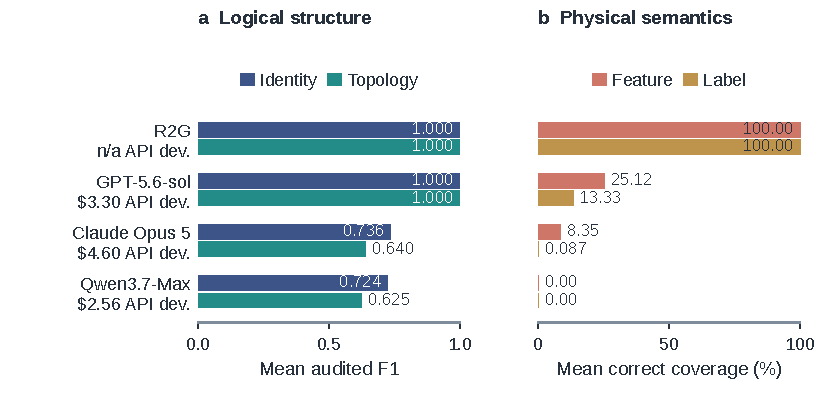
\includegraphics[width=\linewidth]{figures/conversion_semantics.pdf}
\caption{Fixed 24-design conversion benchmark after development under a 600k-token ceiling. Left: identity/topology F1; right: feature/label correct coverage. Model labels include estimated development API USD (Appendix~\ref{app:api_costs}); n/a denotes unmetered tool development. Core acceptance is 24/24 for R2G and 0/24 for each LLM converter.}
\label{fig:conversion}
\end{figure}

\textbf{Topology is necessary but insufficient.} All 96 method--design evaluations complete. R2G passes every core group on all 24 designs, with 1.0 identity/topology F1 and 100\% correct coverage within the audited scope (Fig.~\ref{fig:conversion}). GPT-5.6-sol also attains identity and topology F1 of 1.0; its alignment, mask, and selected causal checks pass on all 24 designs. Its feature and label groups fail on every design, with mean correct coverage of 25.12\% and 13.33\%. Claude Opus 5 reaches identity/topology F1 of 0.7364/0.6400, with 8.35\% feature and 0.087\% label coverage. Qwen3.7-Max reaches 0.7239/0.6247 F1 but provides no verified feature or label coverage. Thus the result distinguishes actual progress in logical reconstruction from completion of the physical supervision interface.

The practical value is an inspectable connection from heterogeneous EDA files to graph inputs and supervision: recovering connectivity alone does not supply stage-valid physical features or correctly associated targets. R2G delivers this connection under the evaluated contract. Appendix~\ref{app:e4} reports development trajectories, detailed check states, and a traced conversion case.

\subsection{Downstream Utility of Stage-Aware Physical Graphs}
\label{sec:downstream}
We test whether the admitted graph fields carry predictive signal rather than merely satisfying a schema. The cohort contains 278 strict-clean designs with a fixed, design-disjoint train/validation/test split of 175/49/54. All reported results use the same 54-design test set and three seeds. GINE models consume topology and numerical features; feature-only MLPs provide a matched non-message-passing baseline. Inputs are restricted to one of four cutoffs---post-synthesis, post-floorplan, post-placement, or post-CTS---and predict common post-route targets. Neither post-route labels nor supervision-only relations enter the encoders. We report test macro MAE, for which lower is better.

\begin{figure}[htbp]
\centering
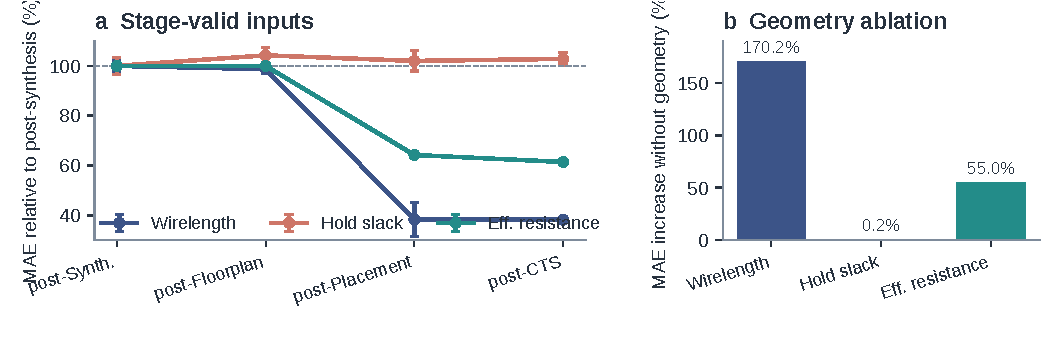
\includegraphics[width=\linewidth]{figures/downstream_utility.pdf}
\caption{Downstream evidence from the fixed 278-design cohort (mean and standard deviation over three seeds). (a) Stage-valid inputs predicting post-route targets, normalized to post-synthesis MAE. (b) Removing geometry from otherwise identical post-placement GINE inputs. Physical stage and geometry information strongly affect wirelength and effective resistance; hold slack is comparatively insensitive.}
\label{fig:downstream}
\end{figure}

Figure~\ref{fig:downstream} shows a sharp information boundary at placement. From post-synthesis to post-placement inputs, wirelength MAE falls from 12.8650 to 4.9321 (61.7\%) and effective-resistance MAE from 14.3060 to 9.1870 (35.8\%). Post-CTS inputs further reach 4.9112 and 8.7820. Removing geometry from post-placement graphs reverses these gains: wirelength MAE rises to 13.3268 (170.2\%) and resistance to 14.2431 (55.0\%). The negligible 0.2\% hold-slack change is an informative negative control rather than evidence of universal benefit.

Topology is likewise target dependent. At post-placement, GINE improves wirelength MAE over the MLP from 7.1548 to 4.9321 and hold-slack MAE from 0.1412 to 0.1316; at post-CTS it improves them from 10.1386 to 4.9112 and from 0.1395 to 0.1327. The MLP is stronger on the other five audited targets. Thus the result is not that one architecture always wins: R2G preserves enough aligned topology, geometry, and supervision to expose which physical targets benefit from each inductive bias.
